\documentclass[declaration,shortabstract, inz]{iithesis}

\usepackage[utf8]{inputenc}

\polishtitle    {Warianty gry w życie Conwaya}
\englishtitle   {Conway's Game of Life variants}
\polishabstract {Przedstawiona praca opisuje implementację projektu, umożliwiającego tworzenie i wizualizację wariantów gry w życie Conwaya opartych na planszy zbudowanej na podstawie diagramów Woronoja. Części składowe projektu to generator diagramów Woronoja oparty na algorytmie S. Fortunea, wizualizacja gry przy zastosowaniu API OpenGl oraz ewaluator języka opisu gry.}
\englishabstract{This paper describes the project, which alowes, creation and visualization of Conway's Game of Life variants, on a a board made of Voronoi diagrams. Project consist of Voronoi diagrams generator using S. Fortune's algoritm, game visualisation using OpenGl API and game description language evaluator.}
\author         {Marcin Rogala}
\advisor        {dr hab. Jan Otop}
\date          {25 grudnia 2020}
\transcriptnum {300084}
\advisorgen    {dr hab. Jan Otopa}


\usepackage{amsmath,amsthm,natbib, caption, mathtools,amsfonts,graphicx,hyperref,listings}
\usepackage[ruled,vlined]{algorithm2e}

\graphicspath{ {./images/} }

\lstdefinestyle{customc}{
  belowcaptionskip=1\baselineskip,
  breaklines=true,
  frame=single,
  xleftmargin=\parindent,
  language=C,
  showstringspaces=false,
  basicstyle=\footnotesize\ttfamily,
  tabsize=3,
}
\lstset{escapechar=@,style=customc}

\theoremstyle{definition} \newtheorem{definition}{Definicja}[]
\theoremstyle{plain} \newtheorem{remark}[definition]{Obserwacja}
\theoremstyle{plain} \newtheorem{theorem}[definition]{Twierdzenie}
\theoremstyle{plain} \newtheorem{example}{Przykład}[definition]
\theoremstyle{plain} \newtheorem{lemma}[definition]{Lemat}

\begin{document}

\chapter{Wprowadzenie}
\section{Gra w życie}
Gra w życie, została zaprezentowana w 1970 roku przez Johna Conwaya na łamach miesięcznika \textit{Scientific American} \cite{gardner}.  Jest~to~gra bez graczy, co oznacza, że jej ewolucja zależy tylko od stanu początkowego bez późniejszych ingerencji człowieka. Planszą jest dwu wymiarowa siatka kwadratowych komórek, z których każda ma 8 sąsiadów. Każda komórka może być żywa lub martwa. W standardowej grze obowiązują tylko trzy reguły:

\begin{itemize}
\item martwa komórka rodzi jeśli ma dokładnie 3 żywych sąsiadów,
\item żywa komórka umiera z zatłoczenia, jeśli ma więcej niż 3 żywych sąsiadów,
\item żywa komórka umiera z samotności jeśli ma mniej niż 2 żywych sąsiadów.
\end{itemize}

Przedstawione przez Conwaya proste zasady pozwoliły zachować równowagę pomiędzy rozrostem i zanikaniem struktur.

Gra w życie ma wiele ciekawych właściwości. Jedną z nich jest równoważność maszynie Turinga, co oznacza, że ma takie same możliwości obliczeniowe jak komputer z nieskończoną pamięcią i brakiem ograniczeń czasowych. Przy użyciu gry~w~życie możliwa jest konstrukcja bramek logicznych oraz implementacja różnych systemów komputerowych. Gra może przebiegać chaotycznie lub według jednego z ustalonych wzorców: 
\begin{itemize}
	\item stabilny -- pozostają niezmienne bez względu na kolejne przekształcenia,
	\item oscylatory -- zmieniają się cyklicznie, regularnie wracają do poprzednich stanów,
	\item statki -- oscylatory zmieniające swoją pozycję na planszy.
\end{itemize}

Gra Conwaya jest przykładem automatu komórkowego, które często wykorzystywane są do przeprowadzania symulacji komputerowych. 
Max Brenner w swoim artykule \cite{brenner} przedstawił symulację rozprzestrzeniania się wirusa COVID-19, co bardzo dobrze pokazuje możliwości, jakie dają nam modyfikacje gry w życie oraz bardziej rozbudowane automaty komórkowe.

\section{Opis projektu}

Przedstawiona praca opisuje projekt pozwalający na definiowanie zasad gry~w~życie, używając prostego języka. Gra odbywa się na planszy będącej diagramem Woronoja, co istotnie narusza jedną z właściwości automatów komórkowych, mianowicie komórki automatu różnią się od siebie. Pozwala to wprowadzić element nieregularności oraz upodabnia grę do prawdziwego życia, w którym elementy symulacji mają istotne różnice wynikające se swojej budowy lub środowiska.
Weźmy za przykład ludzi, którzy mają różną liczbę osób w swoim otoczeniu, co wpływa na wiarygodność symulacji przeprowadzonych na standardowej siatce kwadratów.

\hyperref[sec:fortune]{Pierwszą częścią pracy} jest przedstawienie algorytmu Fortunea pozwalającego na generowanie diagramów Woronoja. Algorytm przyjmuje na wejściu zbiór punktów oraz opierając się na technice zamiatania, generuje na ich podstawie diagram.
Algorytm Fortunea rozpatruje względem współrzędnej $y$ następujące wydarzenia:
\begin{itemize}
	\item site event - miotła napotyka kolejny punkt z wejściowego zbioru,
	\item circle event - miotła napotyka wydarzenie będące niwelacją jednej z paraboli wykorzystywanej do wyznaczania krawędzi diagramu.
\end{itemize}
Po rozpatrzeniu wszystkich wydarzeń wynikiem działania algorytmu są krawędzie oraz graf sąsiedztwa pól diagramu Woronoja.

\hyperref[sec:parser]{Drugą częścią pracy} jest opis gramatyki oraz mechanizmu prasowania i ewaluacji języka opisu gry. Parser tworzonych przez użytkowników programów wykorzystuje bibliotekę PEGTL, która opiera się na gramatycę PEG oraz parsowaniu z góry na dół. Wynikiem parsowania jest abstrakcyjne drzewo rozkładu języka, które jest następnie ewaluowane do odpowiednich funkcji opisujących grę w życie.

\hyperref[sec:openGl]{Kolejna część} to opis wykorzystania API OpenGl do przeprowadzenia wizualizacji gry.

\hyperref[sec:tools]{Pracę uzupełnia opis} istniejących narzędzi i algorytmów do przeprowadzania symulacji z użyciem gry w życie.

\chapter{Diagramy Woronoja}

\section{Definicja}
Niech $S$ będzie skończonym zbiorem parami różnych dwuwymiarowych punktów o współrzędnych rzeczywistych. Punkty zbioru $S$, nazywane będą centrami.

\begin{definition}
	   \textit{Polem diagramu Woronoja} odpowiadającemu punktowi $p \in S$ oznaczamy $Vor_S(p) = \{ x \quad | \quad x 		\in \mathbb{R}^2 \land \forall p' \in S \quad \space dist(x, p) \leq dist(x, p')\}$, gdzie $dist$ oznacza odległość euklidesową dwóch punktów.
\end{definition}

\begin{definition}
	   \textit{Diagram Woronoja}, to zbiór $\{ Vor_S(p) \quad  | \quad p \in S\}$.
\end{definition}

\begin{example}
Przykładowy diagram Woronoja z zaznaczonymi $10$ centrami.
	\begin{center}
		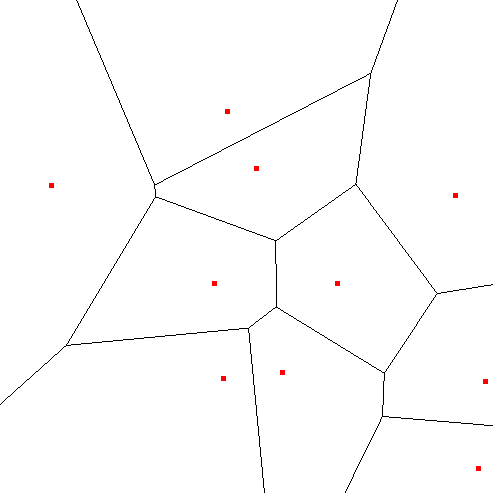
\includegraphics[width=0.7\textwidth]{ExampleDiagram}
	\end{center}
\end{example}

\section{Algorytm Fortunea}
\label{sec:fortune}
\subsection{Opis algorytmu}
Jednym ze sposobów  generowania diagramów Woronoja jest algorytm zaproponowany przez Johna Fortunea oparty na technice zamiatania \cite{miotla}. 

\begin{definition}
\textit{Miotłą} nazywamy poziomą linię poruszającą się od dołu do góry planszy. Wszystkie punkty poniżej miotły zostały już rozpatrzone przez algorytm, natomiast punkty powyżej miotły zostaną rozpatrzone, gdy miotła dojdzie do ich wysokości.
\end{definition}

Najważniejszą strukturą algorytmu jest towarzysząca miotle linia brzegowa. Składa się ona z parabol, rozpinających się nad rozpatrzonymi przez miotłę punktami oraz nieukończonych krawędzi diagramu. W czasie trwania algorytmu parabole rozszerzają się, a ich przecięcia wyznaczają krawędzie. Parabola, która tworzy pole z centrum $p = (x_p, y_p)$ jest zbiorem $\{ x \quad | \quad x \in \mathbb{R}^2 \land dist(p, x) = dist(p_s, x) \}$, gdzie przez $p_s$ oznaczamy punkt na miotle znajdujący się najbliżej $x$. 

\begin{remark}
Punkt przecięcia sąsiednich parabol jest równo odległy od centrów, które definiują te parabole.
\end{remark}

Wyznaczymy wzór $f(x)$ parabol znajdujących się w linii brzegowej.
Niech~$y_s$~oznacza wysokość, na której znajduje się miotła, a $(x_c, y_c)$ będzie centrum pola, które tworzy parabola. 

\begin{align*}
	dist((x_c, y_c), (x, f(x))) &= dist((x, y_s) (x, f(x))) \\
	\sqrt{(x_c - x)^2 + (y_c - f(x))^2} &= \sqrt{(x - x)^2 + (y_s - f(x))^2} \\
	(x_c - x)^2 + (y_c - f(x))^2 &= (y_s - f(x))^2 \\
	(x_c - x)^2 &= (y_s - f(x))^2 - (y_c - f(x))^2 \\ 
	(x_c - x)^2 &= 2f(x)y_c - 2f(x)y_s + y_s^2 - y_c^2 \\
	(x_c - x)^2 + (y_c^2 - y_s^2) &= 2f(x)(y_c - y_s) \\
	f(x) &= \frac{(x - x_c)^2}{2(y_c - y_s)} + \frac{y_c^2 - y_s^2}{2(y_c - y_s)} \\
	f(x) &= \frac{(x - x_c)^2}{2(y_c - y_s)} + \frac{y_c + y_s}{2}
\end{align*}

Korzystając z otrzymanego wzoru, możemy w łatwy sposób wyliczać między innymi przecięcia parabol z innymi obiektami w linii brzegowej.

Poruszająca się przez planszę miotła napotyka dwa rodzaje wydarzeń.

\begin{itemize}
	\item site event -- dotarcie do nowego puntu ze zbioru $S$
	\item circle event -- zniwelowanie jednej z parabol w linii brzegowej
\end{itemize}

\subsubsection{Site event -- obsługa}
\label{sec:site}
Napotykając nowe centrum, musimy dodać do linii brzegowej nową parabolę, dzieląc jedną z istniejących na dwie części. W tym celu przeszukujemy linię brzegową, poszukując paraboli leżącej bezpośrednio pod nowym centrum. To przeszukiwanie będzie miało kluczowy wpływ na złożoność algorytmu. 

\begin{example}
	Zmienione elementy linii brzegowej po obsłużeniu nowego centrum.
	
	\begin{center}
		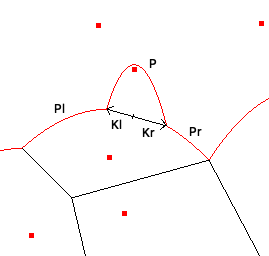
\includegraphics[width=0.6\textwidth]{ExampleSiteEvent}
	\end{center}
\end{example}

Odnaleziona parabola zostaję zastąpiona ciągiem elementów:
\begin{align}
 	P1, K1, P2, K2, P3
\end{align}
Gdzie $P1, P3$ to kopie rozdzielanej paraboli. $P2$ to nowa parabola utworzona przez dodawane centrum. $K1, K2$ to nowe krawędzie rozszerzające się w przeciwnych kierunkach. Punktem startowym dodawanych krawędzi jest punkt na rozdzielanej paraboli znajdujący się pod nowym centrum.

Pozostaje sprawdzić, czy parabole, które dodaliśmy do linii brzegowej, zostaną kiedyś zniwelowane i czy konieczne jest dodanie odpowiednich wydarzeń. 
Parabola zostanie zniwelowana przez swoich sąsiadów, jeśli zachodzą dwa warunki:
\begin{itemize}
	\item parabola nie jest skrajnie lewym lub skrajnie prawym elementem linii brzegowej,
	\item krawędzie (półproste) będące sąsiadami paraboli, przecinają się.
\end{itemize}
Aby dodać nowe wydarzenie polegające na ściśnięciu paraboli przez jej sąsiadów, musimy poznać jego współrzędną $y$. 
Weźmy ciąg elementów linii brzegowej:
\begin{align}
	P1, K1, P2, K2, P3
\end{align}
Punkt $p_i = (x_i, y_i)$ będący punktem przecięcia krawędzi $K1$ i $K2$ jest też miejscem przecięcia parabol $P1$ i $P3$, co czyni $y_i$
wysokością, na której $P2$ zostanie ściśnięte przez $P1$ i $P3$. W tym momencie $p_i$ będzie równo odległe od centrów parabol $P1, P2, P3$. Centra te będą leżały na okręgu o środku $p_i$, skąd wzięła się nazwa wydarzenia.


\subsubsection{Circle event -- obsługa}
\label{sec:circle}
Rozpatrzmy następujący ciąg elementów w linii brzegowej:
\begin{align}
	P1, K1, P2, K2, P3
\end{align}
Załóżmy, że parabola $P2$ zostaje ściśnięta i musimy usunąć ją z linii brzegowej. Leżące po jej bokach krawędzie $K1, K2$ nie będą już rosły. Powinny zostać usunięte i oznaczone jako gotowe krawędzie diagramu. Pozostaje dodać nową krawędź pomiędzy parabolami $P1$ i $P3$ oraz podobnie jak podczas obsługi nowego centrum sprawdzić, czy konieczne jest dodanie wydarzeń niwelacji $P1$ i $P3$.


 \begin{example}
	Obsłużone wydarzenie, usunięto parabolę $P2$ oraz krawędzie $K1, K2$. W ich miejsce dodana została krawędź $K3$.
	
	\begin{center}
		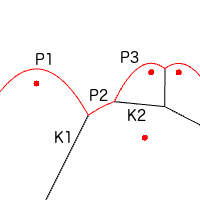
\includegraphics[width=0.4\textwidth]{ExampleCircleEvent1}
		\qquad
		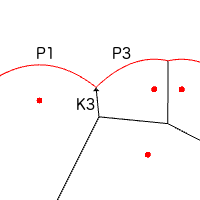
\includegraphics[width=0.4\textwidth]{ExampleCircleEvent2}
	\end{center}
\end{example}

\subsection{Implementacja}

\subsubsection{Pseudokod}
Poniższy pseudokod pokazuje, bardzo uproszczony sposób rozpatrywania wydarzeń. Wydarzenia trzymane są na stosie, zaimplementowanym przy użyciu $priority\_queue$ ze standardowej biblioteki języka $C++$.

\begin{algorithm}[H]
\SetAlgoLined
	Kolejka wydarzeń eventQueue zawiera wszystkie wydarzenia typu site event.\\
 \While{eventQueue nie jest pusta}{
 	currentEvent = eventQueue.top(); \\
  \eIf{currentEvent jest typu site event}{
   		handleSiteEvent(currentEvent);
   }{
   		handleCircleEvent(currentEvent);
  }
 }
 \caption{Pseudokod algorytmu}
\end{algorithm}

\subsubsection{Linia brzegowa}
Linia brzegowa -- \textit{Beachline}, jest najważniejszą strukturą całego algorytmu. Zawiera ona listę struktur \textit{BeachlineField}, przechowującą elementy znajdujące się~w~linii brzegowej. Wszystkie funkcje, których złożoność nie została określona, działają ze stałą złożonością. Najważniejsze funkcje \textit{Beachline} to:

\begin{itemize}
\item \textit{findParabolaForNewSite} -- funkcja wyszukująca parabolę z linii brzegowej, która znajduje się bezpośrednio pod nowym centrum. Funkcja oblicza przecięcia parabol, z ich sąsiadami co pozwala poznać przedział, na jakim się one znajdują. Złożoność tej funkcji to $O(n)$, gdzie $n$ to rozmiar linii brzegowej.

\item \textit{handleSiteEvent} -- funkcja wykonująca niezbędne operacje opisane w \hyperref[sec:site]{Site event -- obsługa}. Złożoność tej funkcji to $O(n)$, gdzie $n$ to rozmiar linii brzegowej.

\item \textit{handleCircleEvent} -- funkcja wykonująca niezbędne operacje opisane w \hyperref[sec:circle]{Circle event -- obsługa}.

\item \textit{addCircleEvents} -- funkcja dodająca niezbędne wydarzenia typu \textit{circle event}, dla nowych elementów linii brzegowej.
\end{itemize}

\textit{Beachline} zawiera dużo funkcji pomocniczych, pomagających obsługiwać wydarzenia oraz wykonywać niezbędne obliczenia na parabolach i krawędziach. Niektóre z tych funkcji to:

\begin{itemize}
\item \textit{addNewField} -- funkcja dodająca nowy element do linii brzegowej,
\item \textit{removeField} -- funkcja usuwająca element z linii brzegowej,
\item \textit{parabolaHalfEdgeIntersection} -- funkcja wyznaczająca punkt przecięcia paraboli z półprostą,
\item \textit{edgesIntersection} -- funkcja wyznaczająca przecięcie półprostych,
\item \textit{completePolygons} -- funkcja czyszcząca linię brzegową po zakończonej pracy oraz oznaczająca ostatnie krawędzie jako zakończone. Złożoność tej funkcji~to~$O(n)$, gdzie~$n$~to~rozmiar linii brzegowej.
\end{itemize}

\textit{Beachline} przechowuje także wynikowe krawędzie algorytmu oraz uzyskany graf połączeń pól diagramu.

\subsubsection{Pozostałe struktury}
\begin{itemize}
	\item \textit{Event} -- przechowuje informacje dotyczące wydarzeń przechowywanych w~\textit{eventQueue},
	\item \textit{Parabola} -- reprezentuje parabolę przechowywaną w linii brzegowej,
	\item \textit{HalfEdge} -- reprezentuję nieukończoną krawędź (półprostą), która rozszerza~się~w~trakcie trwania algorytmu,
	\item \textit{Edge} -- reprezentuje ukończona krawędź.
\end{itemize}

\subsection{Złożoność}
Obsługa każdego wydarzenia typu \textit{site event} dodaje dwie nowe krawędzie oraz dwie nowe parabole do linii brzegowej. Załóżmy, że każda parabola ma przypisane wydarzenie typu \textit{circle event}. Obsługa wydarzenia \textit{circle event} zmniejsza liczbę parabol oraz krawędzi. Oznacza to, że dla $n$ pól diagramu w linii brzegowej będzie $O(n)$ elementów oraz w $eventQueue$ będzie $O(n)$ wydarzeń. Ze względu, na złożoność wyszukiwania parabol w linii brzegowej -- $O(n)$, złożoność całego algorytmu to $O(n^2)$. Możliwe jest osiągnięcie złożoności $O(nlog(n)$, przez zastosowanie zbalansowanego drzewa binarnego do przechowywania elementów linii brzegowej.


\section{Inne algorytmy}

\subsection{Algorytm dziel i zwyciężaj}

Innym podejściem do generowania diagramów Woronoja jest zastosowanie techniki dziel i zwyciężaj. Podczas każdego kroku algorytmu dzielimy zbiór, z którego generujemy diagram na dwa równe, rozłączne podzbiory. Po rekurencyjnym wywołaniu algorytmu i wygenerowaniu diagramu dla mniejszych zbiorów wynikowe diagramy są ze sobą łączone. Złożoność takiego algorytmu to $O(nlogn)$.

\subsection{Algorytm inkrementacyjny}

W tym podejściu do gotowego diagramu Woronoja dodajmemy kolejno nowe punkty, aktualizując istniejący diagram. Początkowo dla jednego punktu diagramem jest ciała płaszczyzna. Złożoność algorytmu to $O(n^2)$.

\subsection{Triangulacja Delone}

\begin{definition}
Triangulacja Delone zbioru $P$ oznaczana jako $DP(P)$ to taka triangulacja, że żaden punkt $p \in P$ nie leży w środku okręgu opisanego na dowolnym trójkącie należącym do $DP(P)$. 
\end{definition}

Algorytmy wyznaczające triangulację Delone działają w złożoności $O(nlogn)$.
Korzystając z wyznaczonej triangulacji, można w łatwy sposób uzyskać diagram Woronoja, łącząc punkty okręgów opisanych na trójkątach. 

\chapter{Język opisu gry}
\label{sec:parser}
Standardową grę w życie można opisać w bardzo prosty sposób. Potrzebne~są~nam informacje o tym, kiedy komórka pozostaje żywa i kiedy ożywa, będąc wcześniej martwa. Możemy z tego wywnioskować, kiedy komórka umiera, co daje nam komplet niezbędnych reguł. Zasady przedstawiamy według następującej konwencji:
\begin{itemize}
\item na początku podajemy liczby żywych sąsiadów, dla których komórka pozostaje żywa,
\item następnie po ukośniku podajemy liczby żywych sąsiadów, dla których komórka ożywa, będąc wcześniej martwa.
\end{itemize}

Podane liczby są mniejsze lub równe $8$, przez co nie ma potrzeby w żaden sposób ich oddzielać.

\begin{example}
$23/3$ to opis zasad gry w życie zaproponowanej przez Conwaya.
\end{example}

Niestety, nieregularność diagramów Woronoja oraz bardziej rozbudowany stan komórek nie pozwala na opisywanie gry w tak prosty sposób. W omawianym projekcie użytkownik definiuje zasady, przy użyciu prostego języka, którego składnia przypomina składnię języka $C$. Takie rozwiązanie pozwala na wykonywanie bardziej skomplikowanych obliczeń podczas przechodzenia między stanami oraz obsługę stanów będących krotkami liczb rzeczywistych, co pozwala na przechowywanie większej ilości informacji o komórce. Użytkownik definiuje także sposób w jaki komórka będzie wyświetlana. Korzystając z bieżącego stanu, określamy jej kolorowanie w postaci \textit{RGB}.

Do zdefiniowania zasad, użytkownik powinien napisać trzy programy. 
\begin{itemize}
\item program \textit{INIT} -- określa początkowe parametry gry. Wywoływany jest tylko raz, przed rozpoczęciem symulacji,
\item program \textit{TRANSITION} -- określa w jaki sposób komórka zmienia swój stan. Wywoływany dla wszystkich komórek podczas każdego kroku gry,
\item program \textit{COLOR} -- określa kolor danego pola, korzystając z jego stanu. Wywoływany dla wszystkich komórek podczas każdego kroku gry, po wykonaniu programu \textit{TRANSITION}.
\end{itemize}

Symulacja gry w życie przebiega w następujący sposób.

\begin{algorithm}[H]
\SetAlgoLined
	Ustaw początkowe parametry, wykonując program \textit{INIT}\\
 \While{licznik kroków jest mniejszy od limitu kroków}{
 	\For{każda komórka}{
 		\textit{TRANSITION} \\
 		\textit{COLOR}	
 	}
 }
 \caption{Pseudokod algorytmu}
\end{algorithm}


\begin{example}
Przykładowy program \textit{INIT} ustawiający kolor początkowy na biały oraz limit kroków na $1000$.
\begin{center}
\begin{lstlisting}
initialColor(1.0, 1.0, 1.0);
stepsLimit(1000);
\end{lstlisting}
\end{center}
\end{example}

\begin{example}
Przykładowy program \textit{TRANSITION} ożywiający komórkę, jeśli ma więcej niż jednego żywego sąsiada.
\begin{center}
\begin{lstlisting}
if(count(0, 1) > 1)
{
	newState[0] = 1;
}
\end{lstlisting}
\end{center}
\end{example}

\begin{example}
Przykładowy program \textit{COLOR} kolorujący żywe komórki na szaro.
\begin{center}
\begin{lstlisting}
if(state[0] == 1)
{
	color[0] = 0.5;
	color[1] = 0.5.
	color[2] = 0.5.
}
\end{lstlisting}
\end{center}
\end{example}

\section{Dane początkowe}
Dane do programu przekazujemy w pliku o rozszerzeniu \textit{.csv}. Pierwszy wiersz pliku zawiera niebędące liczbami nazwy kolumn. Kolejne wiersze zawierają początkowe informacje o komórkach. Pierwsze dwie kolumny każdego wiersza, opisują współrzędne punktów służących do generowania diagramu Woronoja.  Współrzędne muszą zawierać się w przedziale $[-1, 1]$. Kolejne kolumny zawierające dowolne liczby rzeczywiste opisują początkowy stan komórek. Liczba podanych kolumn definiuje rozmiar stanu komórek. Liczby rzeczywiste w pliku wejściowym powinny być zapisane w formacie angielskim -- część ułamkowa oddzielona kropką.

\begin{example}
Przykładowy plik wejściowy opisujący współrzędne punktów oraz stan początkowy zawierający jedną liczbę.
\begin{center}
\begin{tabular}{ |c|c|c| } 
 \hline
 x & y & alive \\
  \hline 
 0.150832 & -0.972647 & 1 \\ 
  \hline
 -0.0799638 & -0.631274 & 0 \\
 \hline
  0.535321 & -0.442343 & 0 \\
 \hline
  0.307639 & -0.247769 & 0 \\
 \hline
  0.704164 & 0.757753 & 1 \\
 \hline
 -0.983095 & -0.128225 & 0 \\
 \hline
 -0.310227 & 0.320775 & 0 \\
 \hline
  -0.998757 & 0.349289 & 1 \\
 \hline
  0.155918 & -0.674355 & 1 \\
 \hline
   0.240373 & 0.8879 & 0 \\
 \hline
\end{tabular}
\end{center}
\end{example}

\section{Konstrukcje językowe}

\subsection{Komentarze}

Użytkownik pisząc programy, może umieścić w nich komentarze. Blok komentarza zaczyna się i kończy znakiem \#. 

\begin{example}
\# Tekst komentarza \#
\end{example}

\subsection{Zmienne}
Zmienne przechowują liczby typu rzeczywistego. Nazwy zmiennych tworzone są, tak jak w języku $C$. Użytkownik nie deklaruje zmiennych,~a~zmienna bez przypisanej wartości ma domyślnie wartość $0$.

\subsection{Atrybuty}
Atrybuty to krotki przechowujące informacje o kolorze i stanie komórek. Dostęp do wartości atrybutów wykonujemy przez operator~$[]$~ do~którego podajemy liczby naturalne z przedziału $[0, n)$, gdzie $n$ to rozmiar atrybutu. Podczas wykonywania napisanych przez użytkownika programów mamy dostęp~do~następujących atrybutów: 
	\begin{itemize}
	\item \textit{color} - krotka o rozmiarze $3$, do której zapisywany jest kolor komórki (RGB), wyznaczony ze stanu w programie, \textit{COLOR}. 
	\item \textit{state} -- krotka z której odczytujemy aktualny stan komórki,
	\item \textit{newState} -- krotka do której zapisujemy wyliczony nowy stan komórki.
	\end{itemize}
Użytkownik nie może wykorzystywać innych atrybutów. Rozmiar \textit{state} i \textit{newState} zależy od dostarczonych do programu danych początkowych. 	

\subsection{Wywołanie funkcji}
Wywołanie funkcji ma następującą formę:
\begin{align}
nazwaFunkcji(argument1,[argument2, \dots])
\end{align}

Argumentami funkcji mogą być liczby rzeczywiste lub naturalne. Wywołanie funkcji może być osobną instrukcją programu (wtedy wartość zwracana przez funkcję jest ignorowana) lub częścią wyrażenia.
Podczas pisania programów, użytkownik ma do dyspozycji przygotowane wcześniej następujące funkcje:
\begin{itemize}
\item \textit{count(index, value)} -- zwraca liczbę sąsiadów komórki, których stan spełnia \textit{state[index] == value}.
\item \textit{random(l, r)} -- zwraca losową liczbę rzeczywistą z przedziału $[l, r]$. Funkcja korzysta z rozkładu jednostajnego.
\item \textit{stepsLimit(limit)} -- ustawia limit kroków do wykonania. Wartość $-1$ oznacza nieskończoność.
\item \textit{initialColor(r, g, b)} -- ustawia początkowy kolor komórek.
\item \textit{printEvery(value)} -- ustawia co ile kroków wygląd planszy jest aktualizowany.
\item \textit{skipState(index, value)} -- przerywa wykonywanie programu \textit{TRANSITION} jeśli zachodzi \textit{state[index] == value}. Dla tego pola pominięte zostanie też wykonanie programu \textit{COLOR}.
\end{itemize}

Jeśli wywołanie funkcji nie jest częścią wyrażenia, musi być zakończone średnikiem.

\subsection{Wyrażenia}
W prezentowanym języku dostępne są operatory binarne: $+, -, * , /, \%, <, >, <=, >=, ==, \&\&, ||$.
Operatory logiczne zwracają wartości $1$ i $0$, oznaczające odpowiednio prawdę i fałsz.
Wyrażeniami mogą być następujące konstrukcje:
\begin{itemize}
\item liczba rzeczywista lub naturalna,
\item wywołanie funkcji,
\item zmienna lub dostęp do wartości atrybutu,
\item operator binarny.
\end{itemize}
Argumentami operatora binarnego mogą być dowolne wyrażenia. Jeśli argumentem operatora binarnego jest inny operator binarny, taki argument musi znajdować~się~w~nawiasach.

\begin{example}
Przykładowe poprawne i błędne wyrażenia:
\begin{itemize}
\item $varName$ -- poprawne wyrażenie,
\item $1 + varName$ -- poprawne wyrażenie,
\item $1.0 + (state[1] + varName)$ -- poprawne wyrażenie,
\item $1 + 2 * 4$ -- błędne wyrażenie, $1 + 2$ lub $2 * 4$ powinno znajdować się w nawiasie.
\end{itemize}
\end{example}

\section{Przypisania}
Wyrażenia możemy przypisywać do zmiennych oraz atrybutów \textit{color} i \textit{newState}. Przypisanie musi być zakończone średnikiem.

\begin{example}
Przykładowe poprawne przypisania:
\begin{itemize}
\item $varName = (1 + varName2) * (10 - varName\_3);$,
\item $color[2] = 0.5;$.
\end{itemize}
\end{example}

\section{Instrukcje warunkowe}
Warunkiem instrukcji $if$, może być dowolne wyrażenie. Blok instrukcji, które zostaną wykonane, jeśli warunek zostanie spełniony, może składać się tylko z instrukcji przypisania i musi być otoczony nawiasami $\{, \}$. Warunek jest spełniony, jeśli wartość wyrażenia jest różna od $0$.

\begin{example}
Przykładowa poprawna instrukcja warunkowa:
\begin{center}
\begin{lstlisting}
if((condVar + 1) == 0)
{
	someVar = 2.0;
	newState[0] = 0;
}
\end{lstlisting}
\end{center}
\end{example}

\section{Opis głównych programów}

\subsection{\textit{INIT}}
Program \textit{INIT} jest miejscem, gdzie przy użyciu funkcji \textit{printEvery, stepsLimit, initialColor} ustawiane są początkowe parametry symulacji.

\subsection{\textit{TRANSITION}}
Program \textit{TRANSITION} służy do definiowania zasad zmiany stanów komórek. Aktualny stan odczytujemy ze zmiennej \textit{state}, która jest automatycznie ustawiana~na~wartości stanu każdej komórki. Wyliczony stan, który będzie aktualny ~w~następnym kroku symulacji zapisujemy do zmiennej \textit{newState}. Domyślnie wartości zmiennej \textit{newState} są takie same jak te w zmiennej \textit{state}.

\subsection{\textit{COLOR}}
Program \textit{COLOR} służy do wyliczania koloru komórek. Korzystając ze zmiennej \textit{state}, wyliczany jest kolor w postaci RGB, który musi zostać zapisany do zmiennej \textit{color}. 

\chapter{Parsowanie i ewaluacja programów}

\section{Wykorzystanie biblioteki PEGTL}
PEGTL to biblioteka pozwalająca na pisanie parserów, dostępna pod licencją MIT. Pozwala ona na proste zdefiniowanie gramatyki języka opisu zasad gry. Przetworzony program przechowywany jest w postaci abstrakcyjnego drzewa rozbioru, wykorzystując dostarczoną w tym celu strukturę. 

Funkcje parsujące oraz definicja gramatyki znajdują się w plikach \textit{Parsing.h} oraz \textit{Parsing.cpp}. 

\section{Gramatyka}

Biblioteka PEGTL pozwala na tworzenie gramatyk przy użyciu prostych reguł:
\begin{itemize}
\item one -- dopasowuje pojedynczy znak,
\item string -- dopasowuje ciąg znaków,
\item seq  -- dopasowuje ciąg zasad,
\item star -- dopasowuje dowolnie długi ciąg jednej reguły,
\item plus -- dopasowuje jedno lub więcej wystąpienie reguły,
\item opt  -- opcjonalne dopasowanie reguły,
\item sor -- wybór pierwszej pasującej reguły w kolejności od lewej.
\end{itemize}

Wszystkie pozostałe dostępne reguły są kombinacjami podanych wyżej. Po zdefiniowaniu gramatyki, jako wejście parsera przekazywany jest ciąg znaków wczytany z plików w katalogu \textit{programs}. Z wczytanych programów usuwane są wszystkie białe znaki, co powoduje, że użytkownik może z nich dowolnie korzystać podczas pisania programów.

\begin{example}
Reguły definiujące liczby.
\begin{center}
\begin{lstlisting}
struct positiveInteger : plus < digit > {};

struct integer : seq <
	opt<one<'-'>>,
	positiveInteger
> {};

struct floatingPoint : seq <
	opt < one < '-' > >,
	plus < digit >,
	one < '.' >,
	plus < digit >
> {};
\end{lstlisting}
\end{center}
\end{example}

\begin{itemize}
\item Dodatnia liczba całkowita zdefiniowana jest przez niepusty ciąg cyfr.
\item Liczba całkowita zdefiniowana jest jako dodatnia liczba całkowita poprzedzona opcjonalnym minusem.
\item Liczba rzeczywista zdefiniowana jest jako opcjonalny minus, po którym następuje niepusty ciąg cyfr, kropka oraz ponownie niepusty ciąg cyfr.
\end{itemize}

\section{Klasy Instruction i Expression}

Abstrakcyjna klasa \textit{Expression} jest podstawą struktury wyrażeń zdefiniowanych w pliku \textit{Evaluation.h}. \textit{Expression} zawiera wirtualną metodę \textit{calculate}, która jest implementowana przez klasy dziedziczące. Pozwala to na łatwe obliczanie wartości rozbudowanych wyrażeń zawartych w programach.

\begin{example}
Klasa dziedzicząca po \textit{Expression} reprezentująca liczbę rzeczy rzeczywistą.
\begin{center}
\begin{lstlisting}
class Number : public Expression {
    float number;
public:
    Number(float num) : number(num) { }
    float calculate()
    {
        return number;
    }
    ~Number() { }
};
\end{lstlisting}
\end{center}
\end{example}

Abstrakcyjna klasa \textit{Instruction}, zawiera wirtualną metod \textit{evaluate}, która jest odpowiedzialna za wykonanie danej instrukcji. Wszystkie klasy dziedziczące po \textit{Instruction} implementują \textit{evaluate}. 

\begin{example}
Klasa dziedzicząca po \textit{Instruction} reprezentująca blok instrukcji do wykonania. \textit{Block} wykorzystywana jest między innymi w klasie reprezentującej instrukcję warunkową.
\begin{center}
\begin{lstlisting}
class Block : public Instruction {
    std::vector<Instruction*> block;
public:
    Block(std::vector<Instruction*> b) : block(b) { }
    void evaluate()
    {
        for(auto ins: block)
            ins->evaluate();
    }
    ~Block() { }
};
\end{lstlisting}
\end{center}
\end{example}

Struktura klas dziedziczących po \textit{Expression} i \textit{Instruction} pozwala na budowanie programów, które zawierają w sobie zasady w jaki sposób mają być wykonane. Dzięki takiemu rozwiązaniu, interpretowanie drzewa zwróconego przez bibliotekę \textit{PEGTL} jest wykonywane tylko raz na początku symulacji. 

\section{Ewaluacja programów}
Po uzyskaniu abstrakcyjnych drzew rozbiorów programów \textit{INIT, TRANSITION, COLOR} zostaną one przetłumaczone na drzewo klas dziedziczących po klasach \textit{Expression} i \textit{Instruction}. Przetłumaczone programy są wywoływane w strukturze \textit{Game}, która odpowiedzialna jest~za~wykonywanie symulacji. Progra, \textit{INIT} ewaluowany jest jednokrotnie, przed rozpoczęciem symulacji. \textit{COLOR} i \textit{TRANSITION} ewaluowane są wielokrotnie, ze atrybutami ustawionymi na dane odpowiadające aktualnie przetwarzanej komórce diagramu. 

Wyrażenia ewaluowane są rekurencyjnie, w sposób gorliwy. Oznacza to, że lewa strona wyrażenia jest wyliczana w całości, przed wyliczeniem prawej strony. Nazwy użytych w programach zmiennych przechowywane są w kontenerze \textit{variable} będącym \textit{unoredered\_map}, ze standardowej biblioteki języka \textit{C++}. Wszystkie przypisane do zmiennych wartości są czyszczone po wykonaniu każdego programu \textit{COLOR} i \textit{TRANSITION}.

\chapter{Wizualizacja}
\label{sec:openGl}
Pierwszym podejściem do wyświetlania symulacji było użycie Legacy OpenGL, który pozwala na wyświetlanie prostych kształtów na ekranie, bez użycia shaderów (programów uruchamianych na karcie graficznej, które opisują w jaki sposób na ekranie wyświetlany jest obraz) i dodatkowych struktur do przesyłania danych. Niestety takie rozwiązanie wiąże się z koniecznością przekazywania kompletu informacji o wyglądzie planszy po każdym kroku symulacji. Jest to bardzo nieefektywne, ponieważ podczas trwania programu kolory wielu pól zmieniają się rzadko, a krawędzie wielokątów pozostają niezmienne. Fakt ten, można wykorzystać stosując Vertex Buffer Object -- VBO, który pozwala na przesłanie danych raz oraz późniejsze aktualizowanie ich jeśli zajdzie taka potrzeba.

Wyświetlanie obrazu podzielone jest na dwie części: wyświetlanie krawędzi wielokątów oraz kolorowanie wielokątów. Dane do wyświetlania ładowane są w funkcji \textit{createBuffers} struktury \textit{Board}, a za aktualizowanie wyglądu planszy, po wykonaniu kroku symulacji, odpowiedzialna  jest funkcja \textit{print}. 

\section{Shadery}

Shadery podzielone są na dwa rodzaje:
\begin{itemize}

\item Vertex shader -- obsługuję wyświetlanie wierzchołków danej figury, określając ich położenie oraz kolor.
\item Fragment shader -- opisuje w jaki sposób wyświetlane jest pole pomiędzy wierzchołkami. Kolor który przekazywany jest na wejściu fragment shadera jest interpolacją koloru wierzchołków figury. W celu uzyskania jednolitego koloru pola, kolor wszystkich wierzchołków musi być taki sam.

\end{itemize}

\section{Wyświetlanie krawędzi}

Krawędzie przekazywane są jako dwa punkty, będące ich końcami. Po zakończeniu generowania diagramu, krawędzie nie są nigdy modyfikowane, dlatego wyświetlane są tylko raz na początku wizualizacji. Za wygląd krawędzi odpowiadają dwa proste shadery. 

\subsection{Vertex shader}
Podstawowy shader ustalający pozycję końców krawędzi.
\begin{center}
\begin{lstlisting}
layout(location = 0) in vec4 position;
void main()
{
	gl_Position = position;
}
\end{lstlisting}
\end{center}

\subsection{Fragment shader}
Shader wyświetlający ciało krawędzi w czarnym kolorze, ignorując kolor wierzchołków.
\begin{center}
\begin{lstlisting}
precision mediump float;
out mediump vec4 color1;
void main()
{
	color1 = vec4(0.0, 0.0, 0.0, 1.0);
}
\end{lstlisting}
\end{center}

\section{Kolorowanie pól diagramu}

Pola diagramów będące wielokątami wypukłymi podzielone zostały na trójkąty. Wierzchołkami każdego z trójkątów są dwa końce jednej z krawędzi oraz punkt będący centrum danego pola. Wielokąt przekazywany jest do VBO jako zbiór trójkątów. Każdy trójkąt reprezentowany jest przez trzy punkty razem z ich kolorami. Podczas trwania symulacji kolory pól ulegają zmianie. W~takim przypadku w VBO aktualizowany jest kolor tylko zmienionych wielokątów, z wykorzystaniem funkcji \textit{glBufferSubData}.

\subsection{Vertex shader}
Shader ustalający pozycję wierzchołków trójkąta oraz ustawiający ich kolor.
\begin{center}
\begin{lstlisting}
layout(location = 0) in vec4 position;
layout(location = 1) in vec3 colorIn1;
precision mediump float;
out mediump vec4 color2;
void main()
{
	gl_Position = position;
	color2 = vec4(colorIn1, 1.0);
}
\end{lstlisting}
\end{center}

\subsection{Fragment shader}
Shader wyświetlający ciało trójkąta w kolorze będącym interpolacją kolorów wierzchołków.
\begin{center}
\begin{lstlisting}
precision mediump float;
in mediump vec4 color2;
out mediump vec4 color3;
void main()
{
	color3 = color2;
}
\end{lstlisting}
\end{center}

\chapter{Przykładowe symulacje}

\section{Pulsujące pierścienie i pechowe pola}

\subsection{Stan}
Stan opisany jest przez dwie liczby.
\begin{itemize}
\item state[0] -- opisuje, czy komórka jest żywa,
\item state[1] -- licznik, mówiący od kiedy komórka powinna być żywa.
\end{itemize}

\subsection{TRANSITION}

\begin{center}
\begin{lstlisting}
cond1 = count(0, 1.0) > 0;
if(cond1 && (random(0.0, 1.0) > 0.5))
{
    newState[0] = 1;
}
if(cond1)
{
    newState[1] = state[1] + 1;
}
if(state[1] > 20)
{
    newState[1] = 0;
    newState[0] = 0;
} 
\end{lstlisting}
\end{center}

Program sprawdza, czy pole ma żywego sąsiada, w takim przypadku startuje licznik oraz  z prawdopodobieństwem $1/2$ ożywia dane pole. Jeśli licznik przekroczy $20$, pole umiera i licznik się zeruje.

\subsection{COLOR}

\begin{center}
\begin{lstlisting}
if(state[0] == 0)
{
    # przypadek 1. #
    color[0] = 1.0;
    color[1] = 1.0;
}
if(state[0])
{
    # przypadek 2. #
    color[0] = 0.1;
    color[1] = 0.8;
}
if((state[1] > 1) && (state[0] == 0))
{
    # przypadek 3. #
    color[0] = 0.9;
    color[1] = 0.0;
}
\end{lstlisting}
\end{center}
Program \textit{COLOR}, rozpatruje trzy przypadki: 
\begin{itemize}
\item pole jest martwe -- kolor biały,
\item pole jest żywe -- kolor niebieski,
\item pole jest martwe, ale od więcej niż jednego kroku powinno być żywe -- kolor fioletowy.
\end{itemize}

\begin{example}
Przykładowy krok symulacji dla $10000$ komórek. Na początku żywe komórki ustawione zostały w $4$ różnych pozycjach.
	\begin{center}
		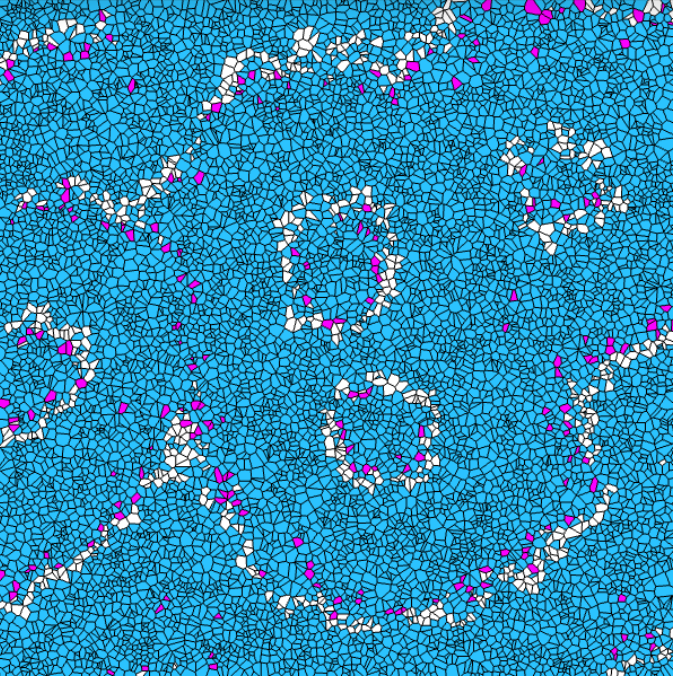
\includegraphics[width=0.6\textwidth]{sim1}
	\end{center}
\end{example}

\section{Zalewanie przeszkód}

\subsection{Stan}
Stan opisany jest przez jedną liczbę -- \textit{state[0]}.
\begin{itemize}
\item state[0] ma wartość 1 -- czy komórka jest żywa,
\item state[0] ma wartość 0 komórka jest martwa.
\item state[0] ma wartość 2 komórka jest przeszkodą.
\end{itemize}

\subsection{INIT}

Program \textit{INIT} wywołuje funkcję \textit{initialColor}, ustawiając kolor początkowy na biały.

\subsection{TRANSITION}

\begin{center}
\begin{lstlisting}
skipState(0, 1);
if(count(0, 1) && (state[0] < 2))
{
	newState[0] = 1;
}
\end{lstlisting}
\end{center}

Program sprawdza, czy pole nie jest przeszkodą i ma żywego sąsiada, w takim przypadku pole ożywa. Jeśli pole jest żywe, pomijane jest wywołanie programu \textit{COLOR}.

\subsection{COLOR}

\begin{center}
\begin{lstlisting}
if(state[0] == 1)
{
	color[0] = 0.0;
	color[1] = 0.0;
}
if(state[0] == 2)
{
	color[0] = 0.5;
	color[1] = 0.5;
	color[2] = 0.5;
}
\end{lstlisting}
\end{center}
Program \textit{COLOR}, rozpatruje trzy przypadki: 
\begin{itemize}
\item pole jest martwe -- kolor biały,
\item pole jest żywe -- kolor niebieski,
\item pole jest przeszkodą -- kolor szary.
\end{itemize}


\begin{example}
Przykładowy krok symulacji dla $50000$ komórek. Przeszkody ułożone zostały w krzyż.	
	
	\begin{center}
		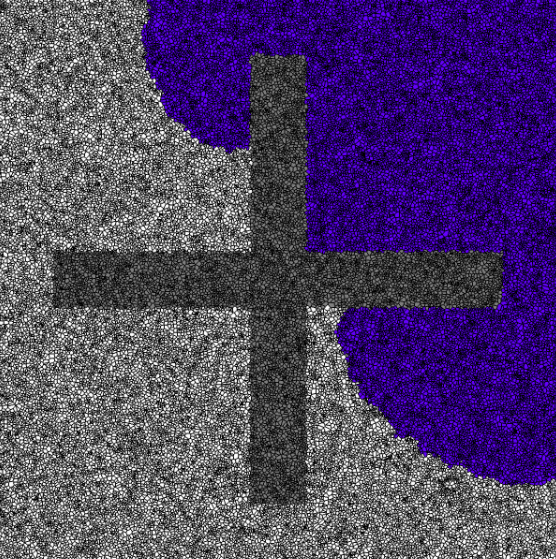
\includegraphics[width=0.6\textwidth]{sim2}
	\end{center}
\end{example}

\section{Różne techniki}
Kolejny przykład demonstruje użycie kilku technik w programie \textit{TRANSITION}. 

Opis stanu:
\begin{itemize}
\item state[0], state[2] -- dyskretny stan pola,
\item state[1] -- losowa właściwości pola,
\item state[3] -- koniunkcja state[0] i state[2], przydatna do użycia zasady włączeń i wyłączeń.
\end{itemize}

\subsection{COLOR}
Program \textit{COLOR} rozpatruje trzy przypadki, przyporządkowując kolory: czerwony, pomarańczowy i żółty.

\begin{center}
\begin{lstlisting}
if((state[0] > 0) && (state[2] == 0))
{
    color[0] = 1.0;
    color[1] = 0.0;
    color[2] = 0.0;
}
if((state[0] > 0) && (state[2] == 1))
{
    color[0] = 1.0;
    color[1] = 0.5;
    color[2] = 0.0;
}
if((state[0] < 1) && (state[2] == 1))
{
    color[0] = 1.0;
    color[1] = 1.0;
    color[2] = 0.0;
}
\end{lstlisting}
\end{center}

\subsection{TRANSITION}
\begin{center}
\begin{lstlisting}
const1 = 0.5;
const2 = 0.1;
const3 = 1.5; 
 
state1 = count(0, 1);
state3 = count(3, 1);
dif = state1 - state3;
 
if((state1 > 0) && (random(0, 1) > const2))
{
    newState[2] = 1;
}
 
ppd = 0.7;
if(state[1] > const1)
{
    ppd = 0.2;
}
 
cond = ((dif + 1.0) * random(0.0, 1.0)) > const3;
 
if(cond && (state[0] == 0))
{
    newState[0] = 1;
}
 
if((state[0] == 1) && (random(0, 1) > const2))
{
    newState[2] = 1;
    newState[3] = 1;
}
\end{lstlisting}
\end{center}

Przydatne techniki:
\begin{itemize}
\item  Deklaracja stałych wartości na początku programu.
\item Użycie dodatkowej wartości w stanie do trzymania koniunkcji wartości.
\item Upraszczanie wyrażeń przez przypisywanie ich części do zmiennych.
\item Losowanie właściwości pola przez podawanie losowych początkowych wartości stanu (podanych w pliku wejściowym).
\end{itemize}

Przedstawiona symulacja jest bardzo podatna na zmiany stałych wartości w programie. Najciekawsze wizualnie efekty uzyskane są przez powyższe ustawienie zmiennych.

\begin{example}
Przykładowy krok symulacji dla $20000$ komórek. Pola koloru pomarańczowego rozprzestrzeniają się w losowych kierunkach.
	\begin{center}
		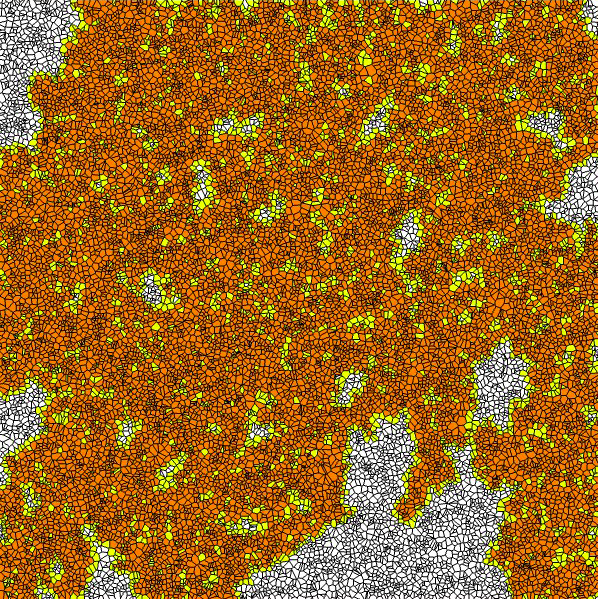
\includegraphics[width=0.6\textwidth]{sim3}
	\end{center}
\end{example}


\chapter{Inne narzędzia}
\label{sec:tools}
Gra w życie zyskała dużą popularność. Od czasu jej publikacji powstało wiele narzędzi pozwalających przeprowadzać symulację różnych jej wariantów. Znaleźć można zarówno bardzo proste, interaktywne narzędzia pozwalające na przedstawienie podstawowych zasad działania gry oraz zaprezentowanie zachodzących zjawisk takich jak oscylatory, jak i zaawansowane programy naukowe, które wykonują tysiące kroków na sekundę i pozwalają w prawie dowolny sposób modyfikować zasady gry.
\section{PlayGameOfLife}
Jest to narzędzie symulujące podstawową grę w życie przedstawioną przez Conwaya. Dane wprowadzane są przez użytkownika ręcznie, zaznaczając żywe pola na interaktywnej planszy. Symulację przeprowadzamy online, pod adresem \url{https://playgameoflife.com/}. Dodatkowe możliwości:
\begin{itemize}
\item modyfikacja planszy w trakcie trwania symulacji
\item zatrzymywanie symulacji i wykonywanie pojedynczych kroków
\item zmiana odstępu czasowego pomiędzy krokami
\end{itemize}

\section{Golly}
Golly \cite{golly}, to narzędzie stworzone do symulacji automatów komórkowych. Skrypty obsługujące symulację są pisane w językach \textit{Python} lub \textit{Lua}. Dzięki zastosowaniu algorytmu \textit{hashlife} \cite{hashlife} Golly jest w stanie przetwarzać duże struktury składające~się~z~milionów komórek. Przykładami pokazującymi możliwości tego narzędzia są zaimplementowane przy jego użyciu systemu komputerowe wykorzystujące równoważność gry w życie z maszyną Turinga \cite{rendell}.


\begin{example}
Maszyna Turinga stworzona przez Paula Rendella.
	\begin{center}
		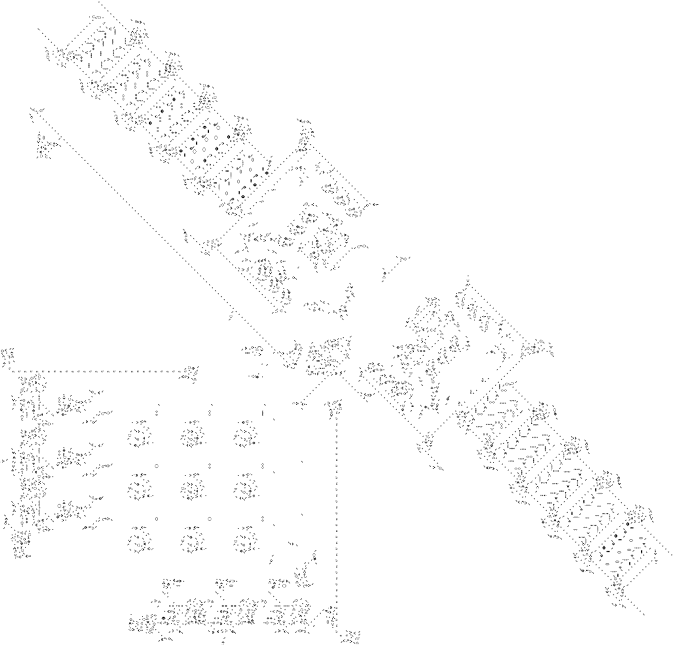
\includegraphics[width=0.7\textwidth]{GollyTuringMachine}
	\end{center}
\end{example}

Golly dostarcza także dużą bibliotekę przykładowych gier w życie, prezentujących jej najciekawsze zachowania.

\begin{example}
Jeden z przykładów zaprezentowanych przez twórców -- gra w życie odbywająca się na planszy złożonej z sześciokątów. 
	\begin{center}
		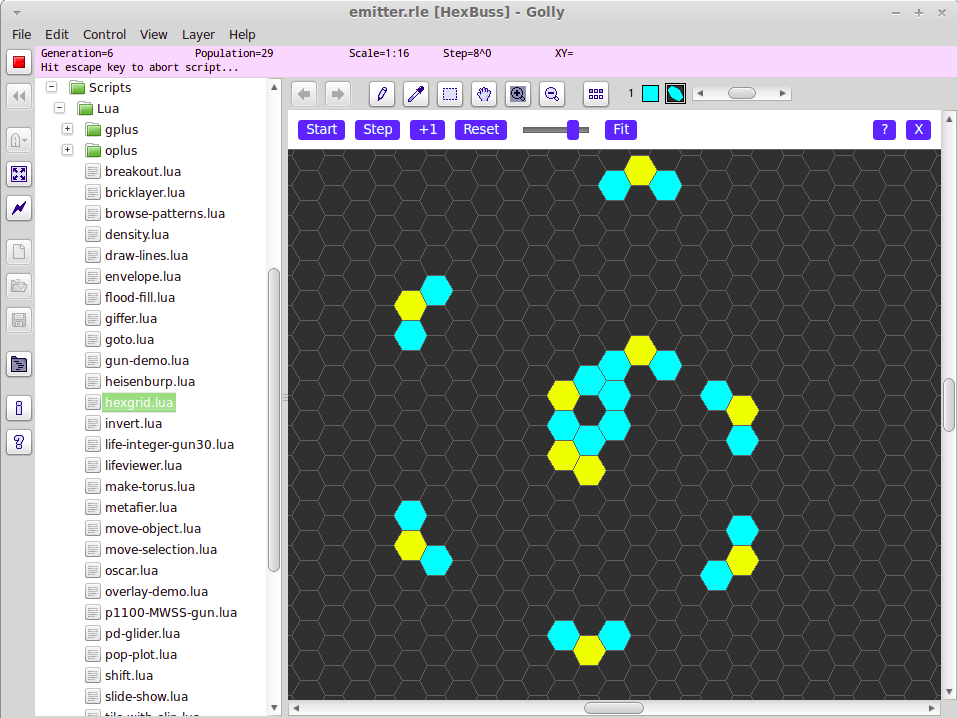
\includegraphics[width=0.7\textwidth]{hexaGolly}
	\end{center}
\end{example}

\subsection{Algorytm hashlife}
Algorytm \textit{hashlife} reprezentuje planszę jako drzewo, którego każdy wierzchołek ma czterech synów. Początkowo plansza dzielona jest na cztery równe kwadratowe części, następnie procedura powtarzana jest dla czterokrotnie mniejszych części planszy. Rozpoznając powtarzające się fragmenty w otrzymanym drzewie, niektóre krawędzie są przepinane w taki sposób, żeby występujące na planszy wzory ułożeń komórek występowały w strukturze tylko raz. Pozwala to zaoszczędzić wykorzystywaną przez algorytm pamięć. Wynik przekształcenia każdego wierzchołka wyliczany jest jednorazowo, a następnie zapamiętywany. Algorytm wykorzystuje ważną własność automatów podobnych do gry w życie. Nawet pozornie losowe struktury automatów komórkowych, mogą zamienić~w~się~zbiór oscylatorów i niezmiennych fragmentów. Istotnymi minusami, są wykorzystywana przez algorytm pamięć oraz początkowy czas działania, niezbędny do zgromadzenia danych o symulacji.

\chapter{Podsumowanie}

\section{Woronoja}
Pierwszą wyzwaniem podczas pracy nad projektem była odpowiednia implementacja algorytmu \textit{Fortunea}, generującego diagramy Woronoja. Niezbędna geometria wymaga wykonywania obliczeń na liczbach rzeczywistych oraz rozpatrzenie wielu przypadków brzegowych. Koncepcja wszystkich obliczeń jest bardzo prosta ale liczba obsługiwanych podczas trwania algorytmu krawędzi i parabol sprawia, że nawet drobny błąd obliczeniowy, może prowadzić do całkowicie zniekształconego diagramu. Obecna wersja implementacji pozwala na bezproblemowe generowanie diagramu posiadającego więcej niż $100000$ pól w czasie kilku sekund. 

\section{Wizualizacja}
Podczas rozbudowywania programu natknąłem się na kolejny duży problem. Pierwsza wersja wizualizacji wykorzystująca \textit{legacy OpenGl} okazała się być zbyt wolna. Symulacja prostej gry na planszy zawierającej kilka tysięcy pól była niepłynna, a oczekiwanie na dalsze kroki zbyt długie. Problem udało się rozwiązać wykorzystując współczesne techniki dostępne w OpenGl. Przesyłanie informacji o wyglądzie planszy tylko w momencie, gdy jest to konieczne pozwoliło osiągnąć płynność nawet dużych symulacji. W tym miejscu pozostaje potencjał do poprawy. Wykorzystując \textit{Vertex Buffer Array}, możliwe jest zredukowanie redundancji przesyłanych danych, co powinno dodatkowo przyśpieszyć wizualizację.

\section{Język opisu gry}
Grę w życie zaprezentowaną przez Conwaya opisują trzy liczby. Taka prosta reprezentacja zasad, utrudniona jest przez nieregularność planszy, dlatego w przedstawionym projekcie, zasady implementowane są w prostym języku opisu gry. Parsowanie przygotowanych przez użytkownika programów, odbywa się przy użyciu biblioteki \textit{PEGTL}. Wynikiem parsowania jest abstrakcyjne drzewo składni języka złożone z dostarczonych struktur. Odpowiednie interpretowanie wynikowego drzewa pozwala na wykonanie programów zawierających reguły gry. Niestety, takie rozwiązanie okazało się być zbyt wolne. Cały zysk, otrzymany przez poprawę wizualizacji, został wykorzystany na interpretowanie programów. 

Proces wykonywania symulacji został przyśpieszony, tłumacząc otrzymane podczas parsowania drzewa, na wewnętrzną reprezentację będącą drzewem opierającym się na dwóch abstrakcyjnych klasach \textit{Expression} i \textit{Instruction} oraz klasach po niech dziedziczących. Takie rozwiązanie pozwala na jednorazowe rozpatrywanie wielu przypadków, niezbędnych do interpretacji programów napisanych przez użytkownika. Po konwersji do nowej reprezentacji, wszystkie informacje potrzebne do wykonania instrukcji, są już dostępne w wierzchołkach drzewa.

Język opisu gry jest też częścią projektu, w której są największe możliwości rozwoju. Dodając nowe reguły do gramatyki parsowanego języka oraz nowe klasy do struktury reprezentującej zinterpretowane drzewo, można w łatwy sposób dodać nowe funkcjonalności. Jednym z przykładów funkcjonalności niewprowadzonych do języka są stałe wartości definiowane w programie \textit{INIT} lub dodatkowe funkcje matematyczne. Oczywiście, możliwości jest więcej i późniejsze rozwijanie zależne jest od potrzeb użytkowników.

\nocite{woronoj}
\bibliographystyle{plain}
\bibliography{bibliography}

\end{document}
